\section{Obnażenie ołtarzy \protect\footnote{W czasie obnażania ołtarza \tt1
        rozpala ogień}}

\begin{itemize}
      \item Do obnażenia ołtarza idziemy w porządku:
            \begin{center}
                  \aa2~~~\aa1\smallskip\\
                  \cc2~~~\cc1\smallskip\\
                  \ii
            \end{center}
      \item Po przyjściu do ołtarza, odebraniu od celebransa biretu i oddaniu
            rewerencji (wszyscy klękają, celebrans się kłania), \cc1 przynosi
            książkę z antyfoną i razem z \cc2 trzymają ją przed \ii
            \footnote{Tekst antyfony w \nameref{sec:dodatek}}.
      \item Zdejmuje się obrus, świece, świeczniki, kwiaty \footnote{Krzyż
                  pozostaje na ołtarzu do Ciemnych Jutrzni. Źródło: F. Małczyński,
                  Ceremoniał obrzędów wielkiego tygodnia, wyd. SS.
                  Loretanek-Benedyktynek, Warszawa, 1958, s. 93.}. Na koniec przewraca
            się świeczniki.
      \item Po zburzeniu świeczników do ołtarza podchodzi \aa1 trzymając tackę z
            ampułkami i \aa2 z ręcznikiem do wytarcia ołtarza.
      \item Po polaniu ołtarza \aa\aa~ odnoszą ręcznik i ampułki. Zostawia się
            szeroko otwarte drzwiczki do tabernakulum.
      \item Gdy X obnaży ołtarz wraca na środek i powtarza antyfonę książki
            trzymanej przez \cc1 i \cc2.
      \item Następnie podchodzi do sedilli gdzie ubiera fioletową kapę. \cc1
            podaje \ii~ biret.
\end{itemize}

\section{Mandatum}

\begin{itemize}
      \item Formuje się procesja na Ewangelię (analogicznie jak w niedzielę).
            \aa\aa~ trzymają zapalone akolitki, które wzięli z kredencji i
            zapalili. (patrz Rys. \ref{fig:mandatum})
            \begin{figure}[h!]
                  \centering
                  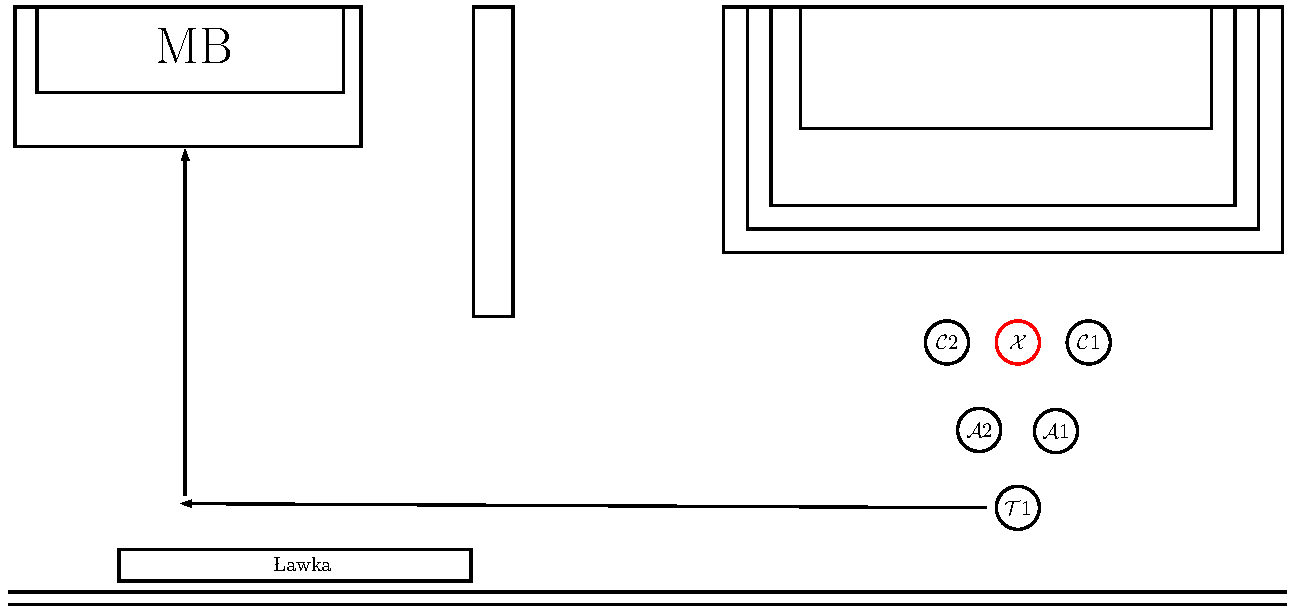
\includegraphics[width=0.8\linewidth]{Figures/Czwartek/Obmycie.pdf}
                  \caption{Procesja do mandatum}
                  \label{fig:mandatum}
            \end{figure}
      \item Po przyjściu do ołtarza bocznego procesja staje na środku.
      \item \aa\aa~ rozchodzą się na boki i robią miejsce dla \ii~ oraz \cc1 i \cc2.
      \item \ii~ oddaje biret, skłania się, podchodzi do ołtarza MB i całuje
            ołtarz
      \item \cc1 i \cc2 wraz z \tt~ stają przed stopniami ołtarzowymi. Następuje
            zasypanie a potem powtórne odczytanie Ewangelii.
      \item Zejście po Ewangelii odbywa się standardowo jak w niedzielę --
            idziemy do małej kredencji.
      \item Po przyjściu \aa\aa~ zostawiają akolitki i przygotowują miednicę i
            dzbanek z wodą.
      \item \cc2 zdejmuje kapę celebransa i podtrzymuje ją w czasie przebierania
            się. \ii~ z pomocą \cc1 zakłada fartuch na fioletową stułę.
      \item \ii~ przebrany w fartuch w asyście \aa\aa~ oraz \cc1 oddają
            rewerencje ołtarzowi i idą do obrzędu mandatum.
      \item W czasie przebierania się \ii~ ministranci wyznaczeniu do mandatum
            podchodzą do umieszczonych tam ławek. Siadają i zdejmują obuwie i
            skarpetkę z prawej nogi.
      \item Po skończeniu przy ołtarzu Matki Bożej \ii~ myje w ciszy ręce.
      \item Po umyciu rąk \ii~ zdejmuje fartuch a zakłada fioletową kapę, (którą
            przynosi \cc2) wchodzi na stopień ołtarza i po stronie Lekcji śpiewa
            w tonie ferialnym \textit{Pater noster} wraz z przepisanymi
            modlitwami. \textbf{Wszyscy stoją}.
      \item Po odmówieniu modlitw przez \ii, skład: \ii, \aa\aa, \cc1 i \cc2 oddają
            rewerencje ołtarzowi i krótką drogą udają się do zakrystii.
      \item Gdy wierni będą opuszczać kościół \cc3 wyprowadza resztę
            ministrantów.
\end{itemize}
